\section{Tricks}






\subsection{FizzleFade}
While most screen transition are done with a black fade effect (by shifting the palette), there are two instances
when the screen transition via fizzling:
\begin{itemize}
	\item When dying
	\item When killing a boss
\end{itemize}


Dying:\\
  \begin{figure}[H] \centering 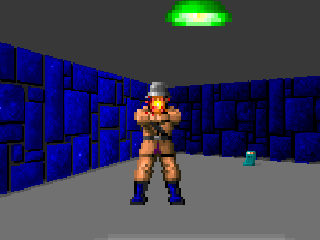
\includegraphics[scale=1.0]{imgs/fizzlefade/dying/screenshot_16.png} \end{figure}
    \begin{figure}[H] \centering 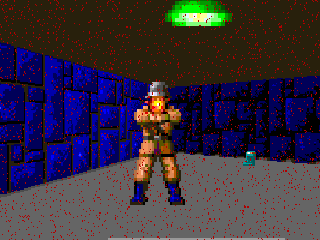
\includegraphics[scale=1.0]{imgs/fizzlefade/dying/screenshot_19.png} \end{figure}
      \begin{figure}[H] \centering 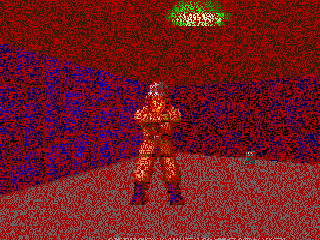
\includegraphics[scale=1.0]{imgs/fizzlefade/dying/screenshot_52.png} \end{figure}
        \begin{figure}[H] \centering 
\includegraphics[scale=1.0]{imgs/fizzlefade/dying/screenshot_86.png} \end{figure}

Boss:\\
\begin{figure}[H] \centering 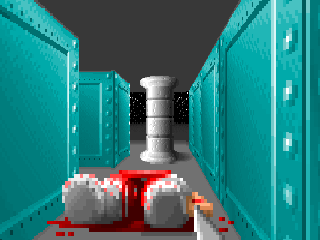
\includegraphics[scale=1.0]{imgs/fizzlefade/boss/screenshot_60.png} \end{figure}        
\begin{figure}[H] \centering 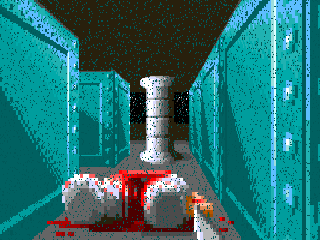
\includegraphics[scale=1.0]{imgs/fizzlefade/boss/screenshot_66.png} \end{figure}        
\begin{figure}[H] \centering 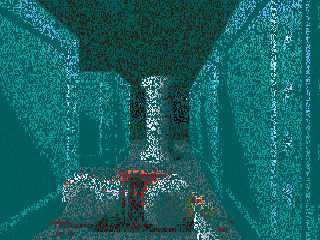
\includegraphics[scale=1.0]{imgs/fizzlefade/boss/screenshot_102.png} \end{figure}        
\begin{figure}[H] \centering 
\includegraphics[scale=1.0]{imgs/fizzlefade/boss/screenshot_130.png} \end{figure}        

The code responsible for this effect can be found in id\_vh.cpp, function FizzleFade. At first it is not obvious to understand how it works. I consider it to be one of the most beautiful trick of the engine:
\newpage
\lstinputlisting[language=C]{code/fizzlefade.c}

        \begin{figure}[H] \centering 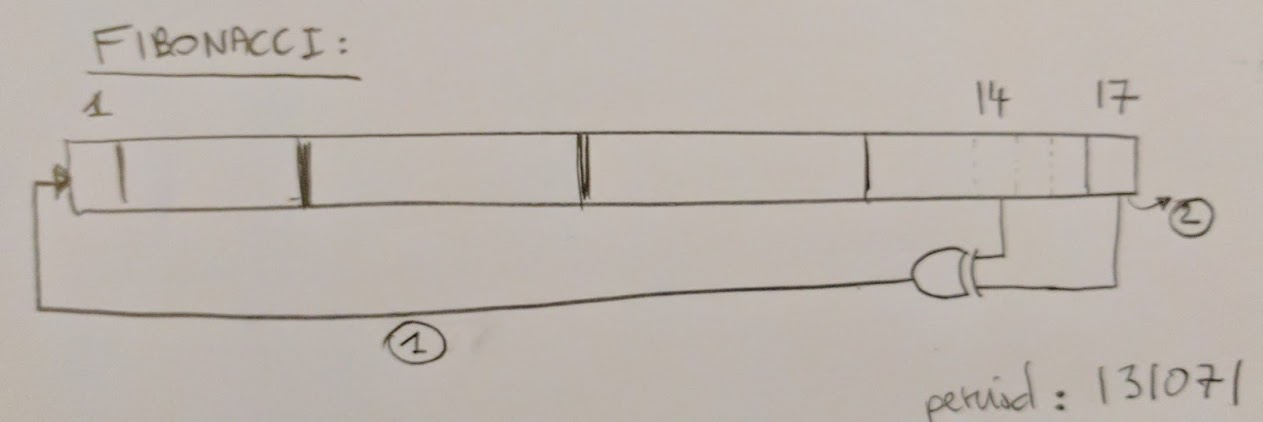
\includegraphics[scale=0.3]{imgs/fizzlefade/fibonnaci.png} \end{figure}
    \begin{figure}[H] \centering 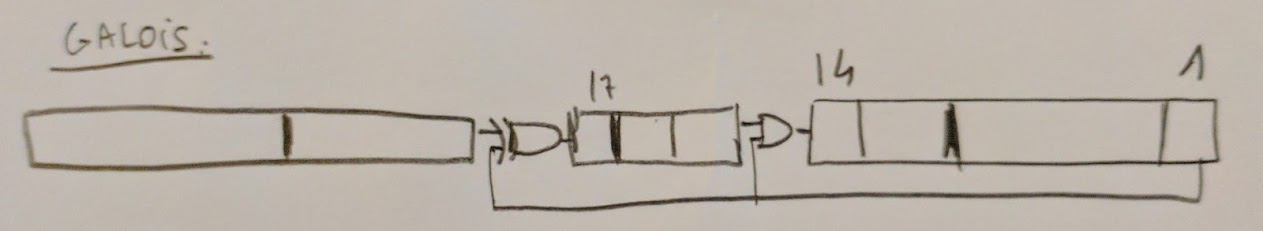
\includegraphics[scale=0.3]{imgs/fizzlefade/galois.png} \end{figure}
      
Note: Because the effect works by plotting pixels individually, this effect was very hard to replicate when developers tried to port the game to hardware accelerated GPU. As far as I know none of the port managed to replicate the fizzlefade.

Note: If you are curious about maximum-length taps, xilinx provides them from 3 to 168\footnote{Xilinx table can be found \href{http://www.xilinx.com/support/documentation/application\_notes/xapp052.pdf}{here}.}.










\subsection{Palette}

Every 1/70th of a second, the VGA output the framebuffer to the screen. Since what is stored are palette index, a translation layer is done in the VGA's DAC. The DAC convert a one byte index to a 3 bytes RGB color. The palette is stored a one block: 256*3 = 768bytes. 
CODE\\
256*3= 768 + setup out operations.\\
This palette allow for fast fading. For example when the played is taking damage, the screen briedly fades to red:
\begin{figure}[H]
  \centering
 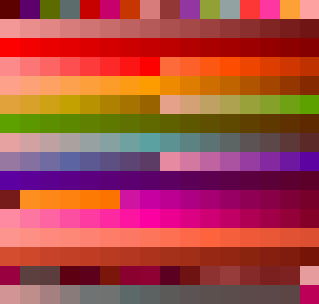
\includegraphics[width=\textwidth]{imgs/palette_damage.png}
 \caption{The palette RGB colors altered when taking damage.} \label{fig:palette_damage}
\end{figure}
There is a trick however: Only the 3D part should fade. UpdatePaletteShifts function.\\
Palette are precomputed in 6 steps toward red or white.\\
What is fast palette setting (via outsb instruction)?\\

\begin{minipage}{\linewidth}
\lstinputlisting[language=C,morekeywords={asm,byte,far}]{code/vl_setpalette.c}
\end{minipage}








\subsection{Cos/Sin table}
To avoid recomputing sin and cos, they are precalculated at startup. Array sintable is initialized as follow:\\
\par

\begin{minipage}{\textwidth}
\lstinputlisting[language=C]{code/sin_cos_table.c}
\end{minipage}


\begin{figure}[H]
 \centering
  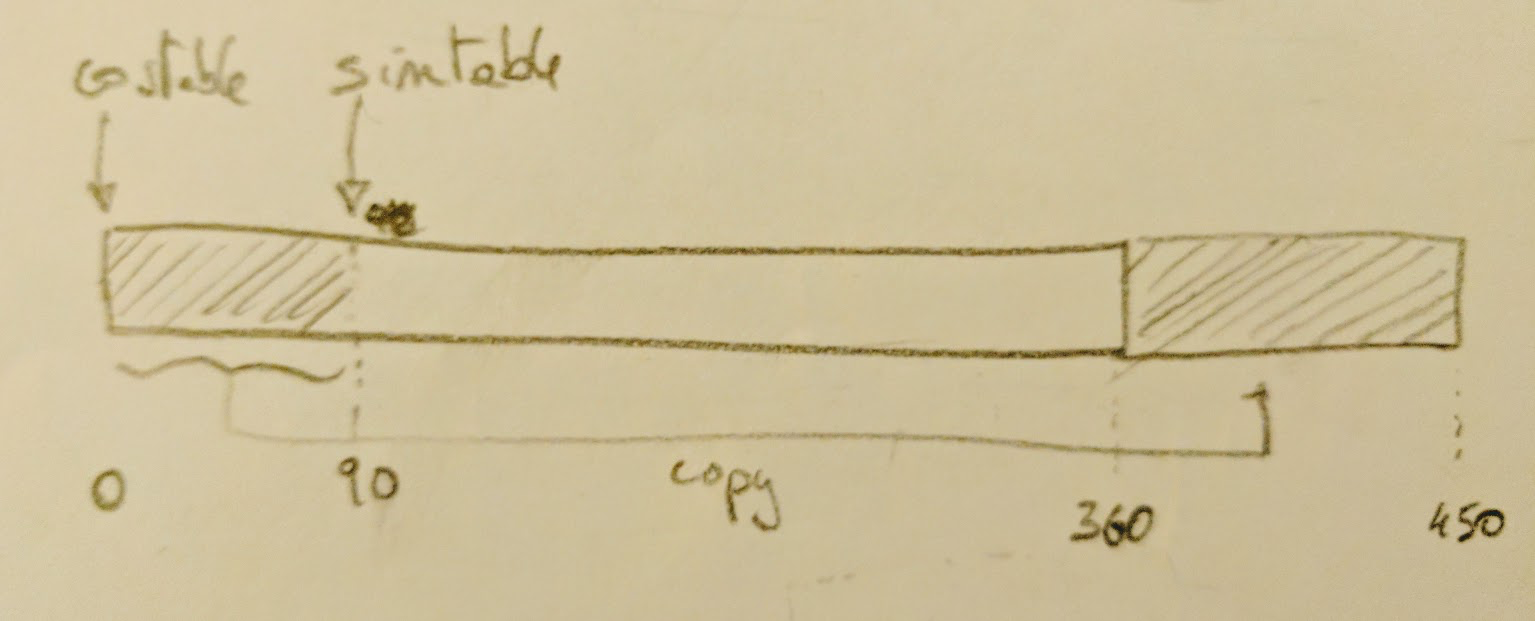
\includegraphics[width=\textwidth]{imgs/cos_sin_table.png}
 \caption{Finalez frame} 
\end{figure}

In order to save space, there is only one array: cos points 90 degres past sin.\\


Trivia: Hard-coded cos and sin lookup table. Budget ?
